\documentclass[handout]{beamer}
%\documentclass{beamer}
{
\usepackage{fullpage}
\usepackage{hyperref}
\usepackage{amssymb} 
}
\usepackage{pgf,pgfarrows,pgfnodes,pgfautomata,pgfheaps,pgfshade}
\usepackage{amsmath,amscd,amssymb}
\usepackage{colortbl}
\usepackage{tikz,pgf,pifont}
\usepackage{mathtools}
\usepackage{pbox}

\usepackage{lstlisting-llvm}
\usepackage[numbered]{mcode}
\usepackage{listings}
\lstloadlanguages{Matlab}
\lstdefinestyle{mcode}{language=MATLAB,escapechar=&}

\usepackage{xcolor}
\usepackage{textcomp}
\usepackage{pgfpages}
\usepackage{hologo}

%\pgfpagesuselayout{4 on 1}[a4paper, border shrink=5mm, landscape]



%\usepackage[latin1]{inputenc}
\usepackage[english]{babel}

  \usetheme{Boadilla}    % Very nice with fewer sections/sub and numbering
  % \usetheme{CambridgeUS}  % Sections and red white + numbers
  % \usetheme{Warsaw}      % Good one no numbers though
  % \usetheme{Darmstadt}   % no University and name
   \setbeamercovered{transparent}
  % \useoutertheme[subsection=true,footnote=false]{miniframes}
  \setbeamertemplate{navigation symbols}{}
  \usecolortheme{crane}

\usepackage{amsmath, amssymb, amsfonts, amsthm,
  verbatim, fancyhdr, graphicx, array, latexsym,
  color, listings, afterpage, epsfig, boxedminipage, 
  fancybox}
\usepackage{amsfonts,amsbsy}


%\usepackage[emtex]{changebar}
%\usepackage{mathptm}  % times+ math
%\usepackage{natbib}
%\usepackage{epsf}
%\usepackage{epsfig}
%\usepackage{rotate}
%\usepackage{amsmath}
%\usepackage{ifthen}
%\usepackage[english]{babel}
% or whatever
%\usepackage[latin1]{inputenc}

% or whatever 
\newcommand{\ud}{\mathrm{d}}
\newcommand{\commentout}[1]{}
\newcommand{\mybox}[1]{\hbox to 0.6\textwidth{#1\hss}}
\newcommand{\pmat}[1]{\begin{pmatrix}#1\end{pmatrix}} 
\newcommand{\red}[1]{\textcolor{red}{#1}}
\newcommand{\blue}[1]{\textcolor{blue}{#1}}
\newcommand{\brown}[1]{\textcolor{brown}{#1}}
\newcommand{\green}[1]{\textcolor{green}{#1}}
\newcommand{\purple}[1]{\textcolor{purple}{#1}}
\newcommand{\gray}[1]{\textcolor{gray}{#1}}


\newcommand{\pder}[2]{\frac{\partial #1}{\partial #2}}
 \newcommand{\norm}[2]{\ensuremath{\| #1 \|_{#2}}}
 \newcommand{\seq}[1]{\ensuremath{\left\{ #1 \right\}}}
 \newcommand{\ipt}[2]{\ensuremath{\left\langle#1,#2\right\rangle}}
 \newcommand{\vbblock}[3]{\ensuremath{\left(\begin{array}{c}\!\!\!#1\\\!\!\!#2\\\!\!\!#3\end{array}\!\!\!\right)}}

 \newcommand{\bblock}[9]{\ensuremath{\left(\begin{array}{ccc}#1&#2&#3\\#4&#5&#6\\#7&#8&#9\end{array}\right)}}
 \def \R{\bb{R}}\def \C{\bb{C}}\def \Z{\bb{Z}}\def \N{\bb{N}}
 \def \a{{\bf a}}
 \def \b{{\bf b}}
 \def \c{{\bf c}}
 \def \d{{\bf d}}
 \def \e{{\bf e}}
 \def \f{{\bf f}}
 \def \g{{\bf g}}
 \def \k{{\bf k}}
 \def \m{{\bf m}}
 \def \n{{\bf n}}
 \def \p{{\bf p}}
 \def \q{{\bf q}}
 \def \r{{\bf r}}
 \def \s{{\bf s}}
 \def \t{{\bf t}}
 \def \u{{\bf u}}
 \def \vv{{\bf v}}
 \def \w{{\bf w}}
 \def \x{{\bf x}}
 \def \y{{\bf y}}
 \def \z{{\bf z}}
 \def \rh{{\alert{h}}}
\def \M{{\cal M}}
\def \L{{\cal L}}
 \def \blambda{{\boldsymbol{\lambda}}}%works with package amsbsy
\newcommand{\hnorm}[2]{\ensuremath{| #1 |_{#2}}}
\newcommand{\ip}[2]{\ensuremath{\left(#1,#2\right)}}




\definecolor{Brown}{cmyk}{0,0.81,1,0.60}
\definecolor{Green}{rgb}{0.516, 0.5976, 0.480}
\definecolor{OliveGreen}{cmyk}{0.64,0,0.95,0.40}
\definecolor{CadetBlue}{rgb}{0.17,0.30,0.547}
\definecolor{Red}{rgb}{0.684,0.156,0.32}
\lstset{
  language=matlab,
  basicstyle=\ttfamily,
  frame=ltrb,
  framesep=5pt,
  basicstyle=\scriptsize,
  stringstyle=\ttfamily\color{Brown}\bfseries,
  commentstyle=\ttfamily\color{Green}\bfseries,
  keywordstyle=\ttfamily\color{CadetBlue}\bfseries,
  identifierstyle=\ttfamily, 
  tabsize=2,
  showstringspaces=true,
  numbers=none
}




%%%%%%%%%%%%%%%%%%%%%%%%%%%%%%%%%%%%%%%%%%%%%%%%%%%%%%%%%%%%%%%%%%%%%%
%%%%%%%%%%%%%%%%%%%%%%%%%%%%%%%%%%%%%%%%%%%%%%%%%%%%%%%%%%%%%%%%%%%%%%
%%%%%%%%%%%%%%%%%%%%%%%%%%%%%%%%%%%%%%%%%%%%%%%%%%%%%%%%%%%%%%%%%%%%%%

% slide 1:
% ========

% title and affiliation

\title[PDE LAB6, 2015]{Master of Science on Computational Science}



\author[prof. Dr. Rolf Krause \& Dr. Drosos Kourounis] % (optional, use only with lots of authors)
{\textbf{Institute of Computational Science}}
% - Give the names in the same order as the appear in the paper.
% - Use the \inst{?} command only if the authors have different
%   affiliation.

\institute[ICS] % (optional, but mostly needed)
{
prof. Dr. Rolf Krause \& Dr. Drosos Kourounis
}
% If you have a file called "university-logo-filename.xxx", where xxx
% is a graphic format that can be processed by latex or pdflatex,
% resp., then you can add a logo as follows:


%\pgfdeclareimage[height=1.0cm]{university-logo}{uoi}
%\logo{\pgfuseimage{university-logo}}

% - Use the \inst command only if there are several affiliations.
% - Keep it simple, no one is interested in your street address.

\date[29 Oct, 2015]{29 Oct 2015, LAB7}

\usefonttheme{serif}


\AtBeginSubsection[]
{
  \begin{frame}<beamer>
    \frametitle{Outline}
    \tableofcontents[currentsection,currentsubsection]
  \end{frame}
}
\setbeamertemplate{footline}
{
  \begin{beamercolorbox}[colsep=1.5pt]{upper separation line foot}
  \end{beamercolorbox}
  \begin{beamercolorbox}[ht=2.5ex,dp=1.125ex,%
    leftskip=.3cm,rightskip=.3cm plus1fil]{title in head/foot}%
    \leavevmode{\usebeamerfont{title in head/foot}
      \insertsection \hfill \insertsubsection\ \hfill \insertshorttitle}%
  \end{beamercolorbox}%
  \begin{beamercolorbox}[colsep=1.5pt]{lower separation line foot}
  \end{beamercolorbox}
}



\begin{document}


\begin{frame}
  \titlepage
\end{frame}

\section{Finite Elements for 3D tetrahedra}


\begin{frame}{The linear system}
\begin{block}{After discretization in space or space and time we end up with}
\begin{align*}
           A\: x &= b, \quad \text{or in the time dependent case}, \\
           A_n\: x_n &= b_n
\end{align*}
\end{block}

\begin{block}{Solution techniques}
\begin{itemize}
\item Direct sparse methods
\item Iterative methods
\end{itemize}
\end{block}
\end{frame}


\subsection{Direct sparse methods}

\begin{frame}{Direct sparse solvers}

\begin{center}

\begin{minipage}{0.45\textwidth}
\begin{block}{Complexity in 2D}
  \begin{itemize}
  \item O($N^{1.5}$) factorization 
  \item O($N \log N$) solution
  \end{itemize}  
\end{block}
\end{minipage}
\hfill
\begin{minipage}{0.45\textwidth}
\begin{block}{Complexity in 3D}
  \begin{itemize}
  \item \red{O($N^{2}$) factorization}
  \item O($N^{1.5}$) solution
  \end{itemize}  
\end{block}
\end{minipage}

\bigskip

\bigskip

\begin{minipage}{0.6\textwidth}
Available Software
{\small
  \begin{itemize}
  \item \blue{PARDISO}
  \item UMFPACK, CHOLMOD
  \item SUPERLU
  \item MUMPS
  \end{itemize}  
}
\end{minipage}

\end{center}

\end{frame}

\begin{frame}{Efficient linear algebra}
   \begin{center}
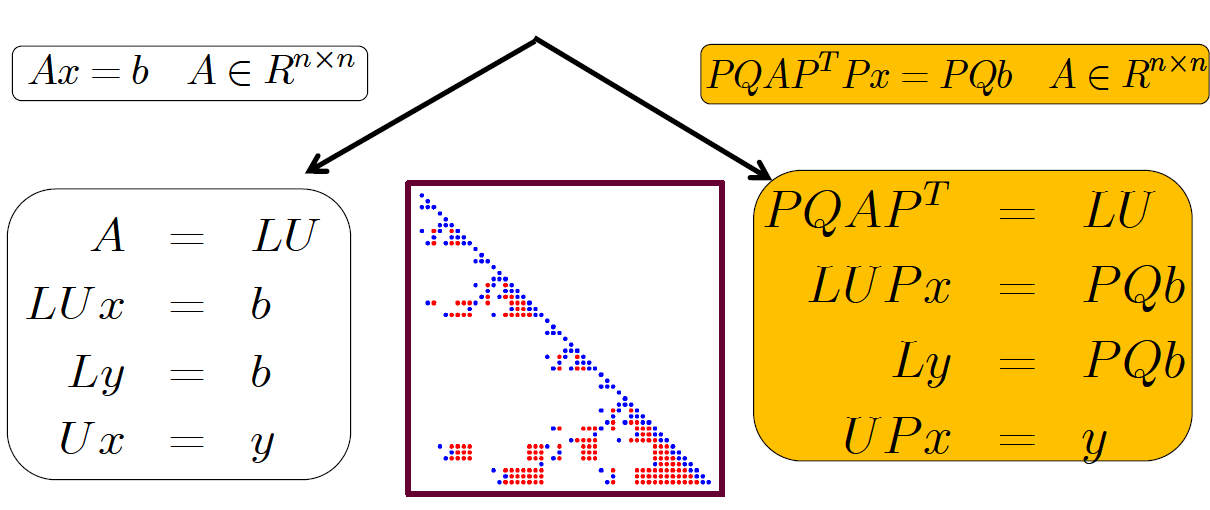
\includegraphics[width=0.90\linewidth]{figures/lu.png}
    \end{center}

\begin{itemize}
\item Permutations $P$ and $Q$ chosen to preserve 
\textbf{\blue sparsity} and \textbf{\blue maintain stability} in $P A Q = LU$.
\item $L$ =  Lower triangular, $U$ = Upper triangular (\textbf{\blue sparse})

\end{itemize}
\end{frame}




\begin{frame}{Nested dissection permutation $P$} 
  \begin{center}
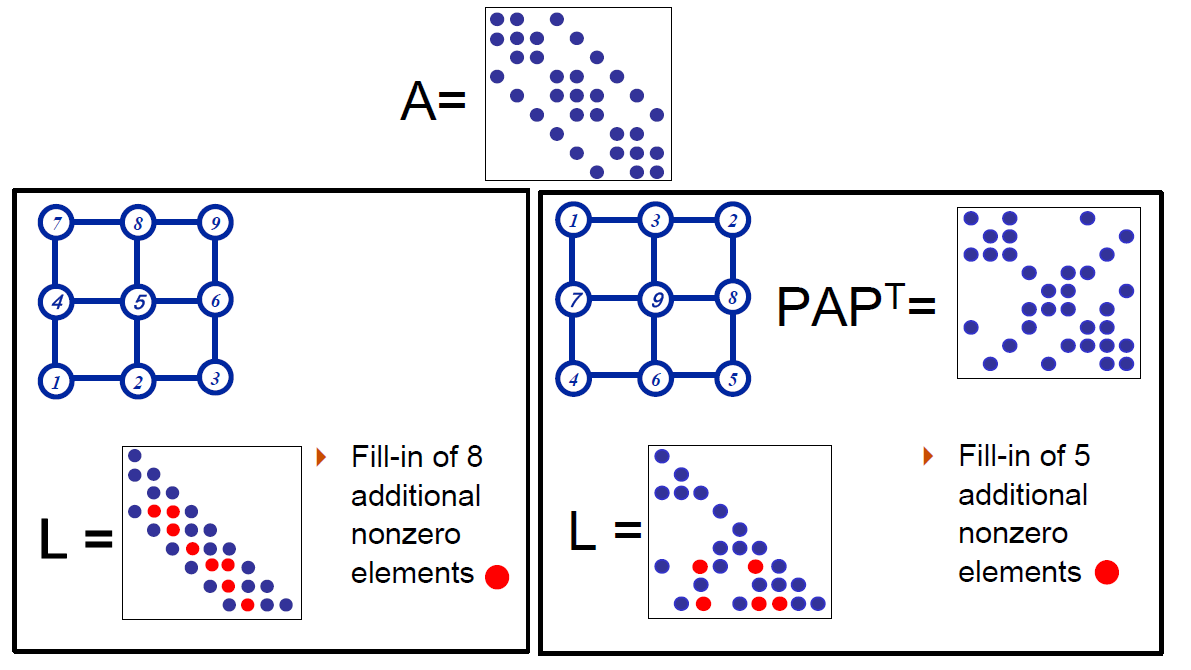
\includegraphics[width=0.95\linewidth]{figures/mrtis2.png}
    \end{center}
\end{frame}




\begin{frame}{Nested dissection ordering on a $7 \times 7$ grid} 
  \begin{center}
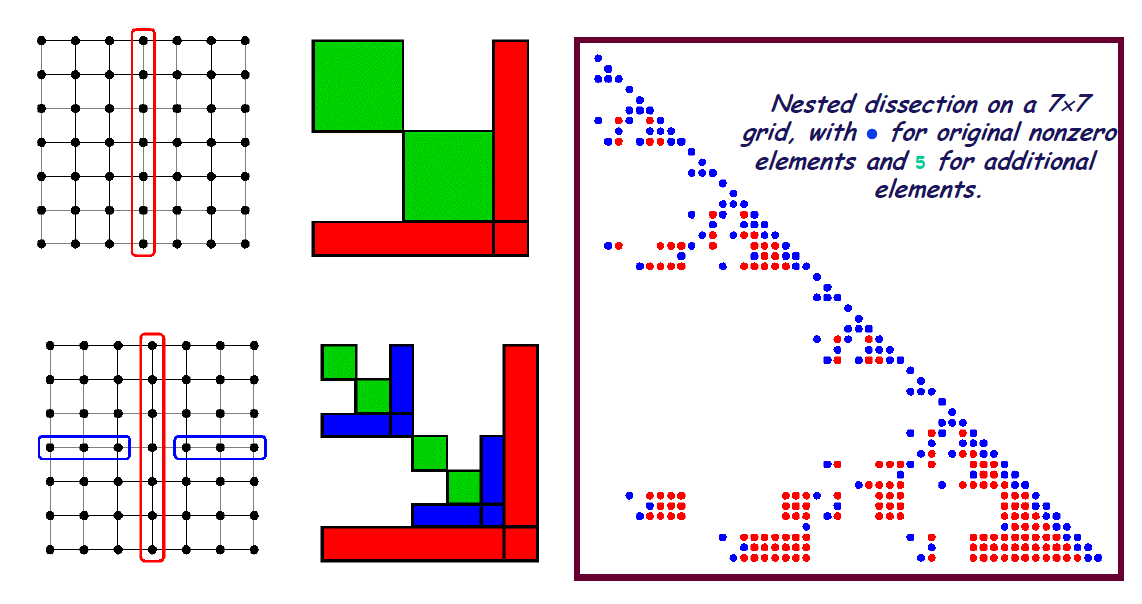
\includegraphics[width=0.90\linewidth]{figures/fill4.png}
    \end{center}
\end{frame}

\begin{frame}
\frametitle{Direct Sparse Solvers}
\begin{block}{PARDISO performance in 2D}
\begin{table}
\centering
\begin{tabular}{||r||r|r|r|r||r||}
  \hline
  \multicolumn{1}{||c||}{mesh}
      & \multicolumn{4}{c||}{Elapsed time in seconds}
      & \multicolumn{1}{c||}{memory} \\
  \hline
  nodes & init & fact & back-sub & total & MB~~~\\
  \hline
%     4014& 0.037 & 0.011 & \blue{0.001~} & 0.049 & \red{  1.4~~} \\
%    16454& 0.158 & 0.052 & \blue{0.004~} & 0.216 & \red{  5.9~~} \\
    65175& 0.704 & 0.265 & \blue{0.019~} & 0.988 & \red{ 26.0~~} \\
   263838& 3.199 & 1.539 & \blue{0.111~} & 4.849 & \red{117.5~~} \\
  1068112& 14.766& 9.518 & \blue{0.535~} &24.819 & \red{527.7~~} \\
  \hline
\end{tabular}
\end{table}
\end{block}

\begin{block}{PARDISO performance in 3D}
\begin{table}
\centering
\begin{tabular}{||r||r|r|r|r||r||}
  \hline
  \multicolumn{1}{||c||}{mesh}
      & \multicolumn{4}{c||}{Elapsed time in seconds}
      & \multicolumn{1}{c||}{memory} \\
  \hline
  nodes   & init & fact & back-sub & total & MB~~~ \\
  \hline
%      500 &  0.005 &    0.001 & \blue{0~}     & 0.006 & \red{    0.3~} \\ 
%     4001 &  0.062 &    0.057 & \blue{0.002~} & 0.121 & \red{    4.7~} \\
    32002 &  0.636 &    2.783 & \blue{0.069~} & 3.488 & \red{   80.4~} \\
   256011 &  6.925 &  185.469 & \blue{1.428~} & 193.8 & \red{ 1438.3~} \\
  2000396 & 76.625 & 11762.1  & \blue{21.46~} & 11860 & \red{24403.0~}  \\
  \hline
\end{tabular}
\end{table}
\end{block}


\end{frame}


\subsection{Iterative methods}

\begin{frame}
\frametitle{Iterative Krylov subspace methods}

They work with matrix-vector products $Ay$ for given vectors $y$
\begin{columns}[t]
\column{.45\textwidth}
\begin{block}{Symmetric systems}
\begin{itemize}
\item \blue{\bf{PCG}}
\item \blue{\bf{MINRES}}
\item \blue{\bf{SYMMLQ}}
\item \blue{\bf{LSMR}}
\item \blue{\bf{SQMR}}
\end{itemize}
\end{block}

\column{.45\textwidth}
\begin{block}{Nonsymmetric systems}
\begin{itemize}
\item \red{\bf{GMRES}}
\item \red{\bf{CGS}}
\item \red{\bf{BICGSTAB}}
\item \red{\bf{QMR}}
\item \red{\bf{LSQR}}
\end{itemize}
\end{block}
\end{columns}

\pause

\begin{block}{Preconditioners}
\vskip-.5cm
\begin{align*}
           A\: x &= b
\\ \text{left:} \quad P^{-1} A \: x &= P^{-1} b
\\ \text{right:} \quad A P^{-1} \: y &= b, \quad P \: x = y
\end{align*}
\end{block}

\end{frame}


\begin{frame}{Iterative Krylov subspace methods}
 At each timestep of the simulation whether we solve linear or nonlinear 
 PDEs we need to solve until convergence one or several linear systems:
\begin{center}
 \begin{minipage}{0.45\textwidth}
 \begin{block}{At the $n$th timestep}
\begin{align*}
 A_n \; x_n = b_n
\end{align*}
\end{block}
\end{minipage}
\hfill
\begin{minipage}{0.45\textwidth}
\begin{block}{Left preconditioning}
\begin{align*}
P_n^{-1} (A_n \; x_n) = P_n^{-1} \; b_n
\end{align*}
\end{block}
\end{minipage}

\medskip

 \begin{minipage}{0.45\textwidth}
\begin{block}{}
High condition number
\end{block}
\end{minipage}
\hfill
 \begin{minipage}{0.45\textwidth}
\begin{block}{}
Lower condition number
\end{block}
\end{minipage}

\medskip
\pause
Iterative Krylov subspace methods require only matrix-vector 
products $Ay$ for given vectors $y$ and depending on the type
of the matrix we have

\begin{columns}[t]
\column{.45\textwidth}
\begin{block}{Symmetric matrices}
\begin{itemize}
\item \blue{\bf{PCG}}
\item \blue{\bf{MINRES}}
\end{itemize}
\end{block}

\column{.45\textwidth}
\begin{block}{Nonsymmetric matrices}
\begin{itemize}
\item \red{\bf{GMRES}}
\item \red{\bf{BICGSTAB}}
\end{itemize}
\end{block}
\end{columns}


\end{center}
\end{frame}


\begin{frame}{Generalized minimum residual methods}
\centering
\footnotesize{
\begin{minipage}{0.48\linewidth}
\begin{block}{\footnotesize {\textcolor{blue}{GMRES}(A,M,b,tol)}}
\vspace{-0.5cm}
\begin{align*}
   &x_0 = M^{-1}b, \; r_0 = b - Ax_0, \\ 
   &\beta = \Vert r_0 \Vert_2 \; u_1 = \frac{r_0}{\beta}, \; k = 0 \\
   &\text{while} \quad \Vert r_k \Vert_2 > \beta \; tol  \\
   &\quad k = k + 1 \; \blue{z_k = M^{-1} v_k, \; w = Az_k} \\
   &\quad \text{for} \; i = 1,2,\ldots,k \; \text{do} \\
   &\quad \quad h_{i,k} = u_i^T w, \; w = w - h_{i,k} u_i \\
   &\quad \text{end for} \\
   &\quad h_{k+1,k} = \Vert w \Vert_2, \; u_{k+1} = \frac{w}{h_{k+1,k}} \\
   &\quad V_k = [v_1, \ldots, v_k] \\ 
   &\quad H_k = \{h_{i,j}\}, \; 1\le i \le j+1, \; 1 \le j \le k \\
   &\quad y_k = \text{argmin}_y \Vert \beta e_1 - H_k \:  y \Vert_2 \\
   &\quad \textcolor{blue}{x_k = x_0 + M^{-1} V_k \: y_k}, \; r_k = b-A \: x_k \\
   &\text{end while}
\end{align*}
\end{block}
\end{minipage}
\hfill
\begin{minipage}{0.48\linewidth}
\begin{block}{\footnotesize {\textcolor{red}{FGMRES}(A,M,b,tol)}}
\vspace{-0.5cm}
\begin{align*}
   &x_0 = M^{-1}_0b, \; r_0 = b - Ax_0, \\ 
   &\beta = \Vert r_0 \Vert_2 \; u_1 = \frac{r_0}{\beta}, \; k = 0 \\
   &\text{while} \quad \Vert r_k \Vert_2 > \beta \; tol  \\
   &\quad k = k + 1, z_k = M^{-1}_k v_k, \; w = Az_k \\
   &\quad \text{for} \; i = 1,2,\ldots,k \; \text{do} \\
   &\quad \quad h_{i,k} = u_i^T w, \; w = w - h_{i,k} u_i \\
   &\quad \text{end for} \\
   &\quad h_{k+1,k} = \Vert w \Vert_2, \; u_{k+1} = \frac{w}{h_{k+1,k}} \\
   &\quad V_k = [v_1, \ldots, v_k], \; \textcolor{red}{Z_k = [z_1, \ldots, z_k]} \\ 
   &\quad H_k = \{h_{i,j}\}, \; 1\le i \le j+1, \; 1 \le j \le k \\
   &\quad y_k = \text{argmin}_y \Vert \beta e_1 - H_k \:  y \Vert_2 \\
   &\quad \textcolor{red}{x_k = x_0 + Z_k \: y_k}, \; r_k = b-A \: x_k \\
   &\text{end while}
\end{align*}
\end{block}
\end{minipage}
}
\end{frame}



\begin{frame}
\frametitle{Preconditioning methods: domain decomposition}

\begin{center}
  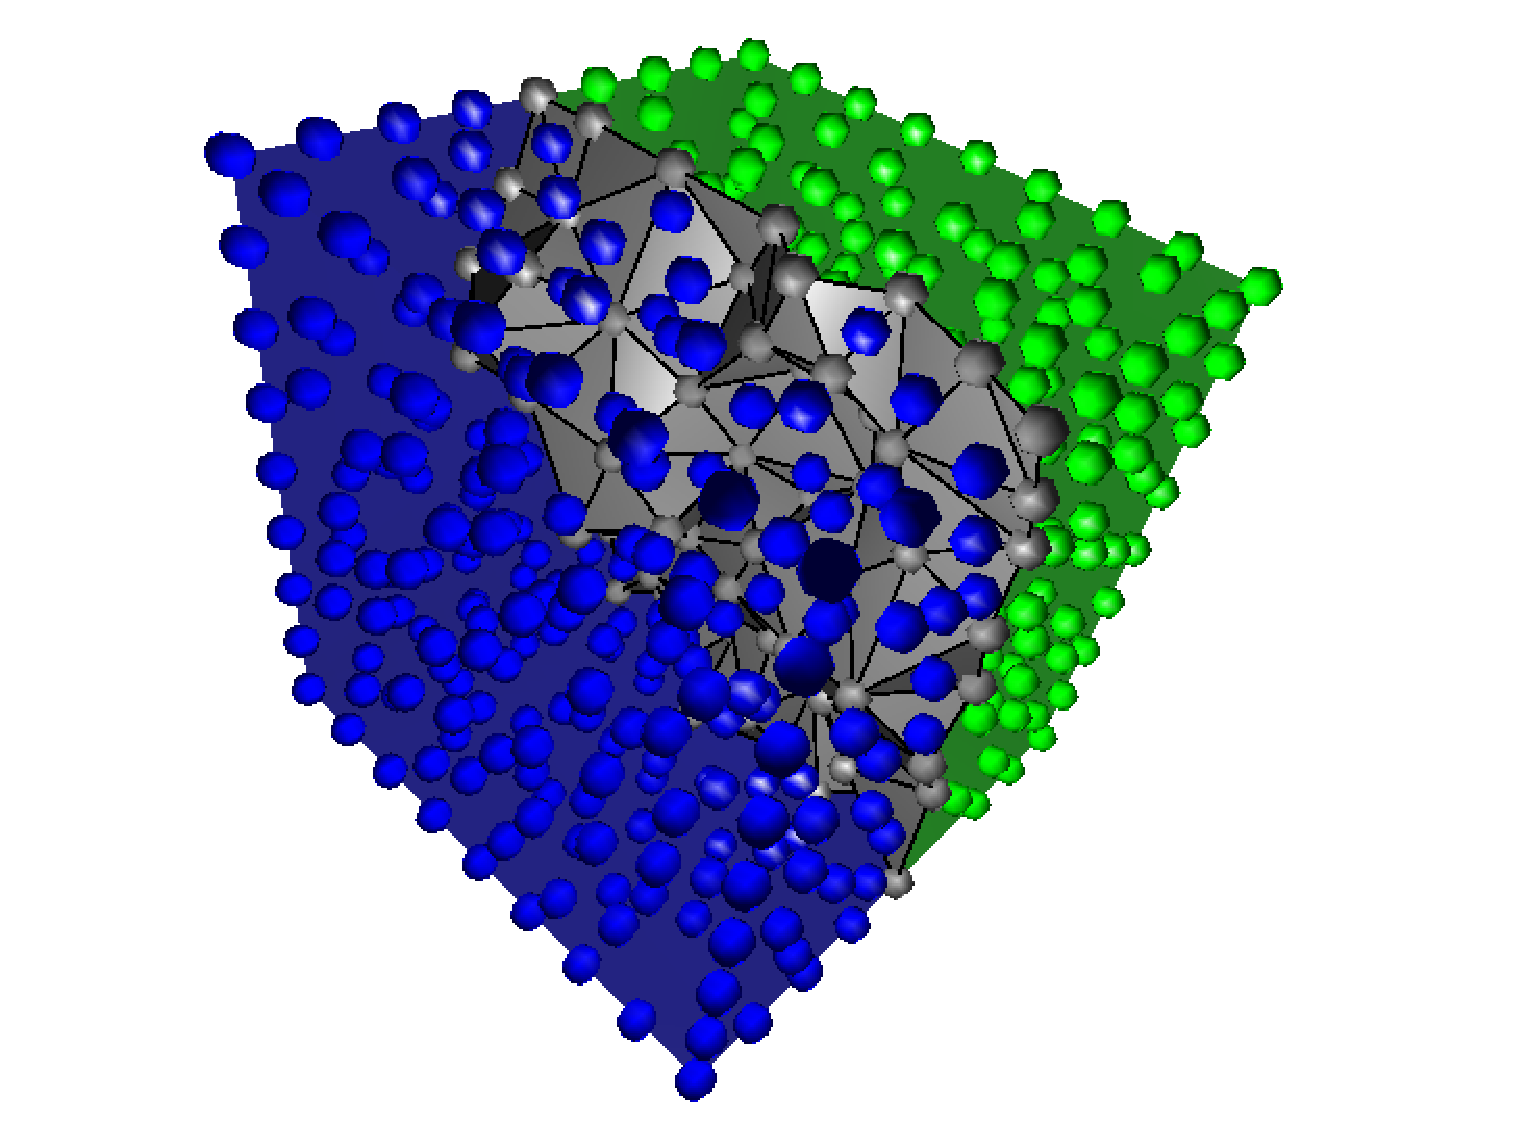
\includegraphics[width=6.0cm]{figures/3Ddomain-2parts.pdf}
  \hspace*{-1.0cm}
  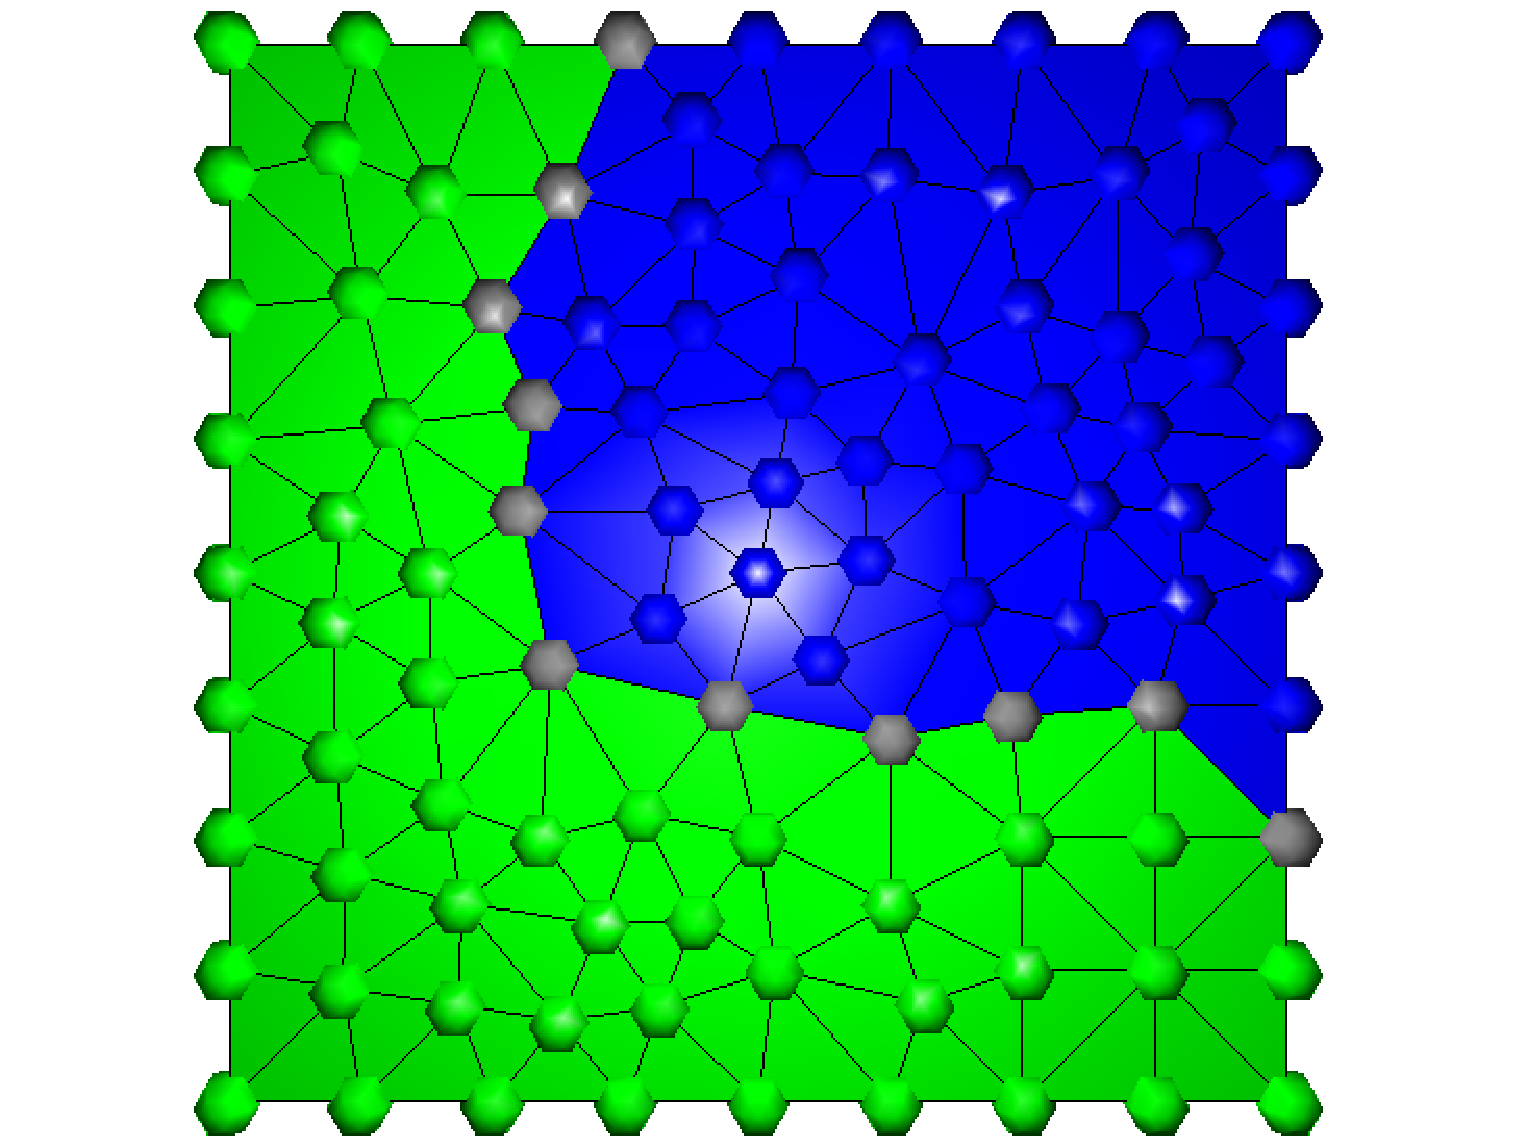
\includegraphics[width=6.0cm]{figures/2subdomain.pdf}
\end{center}
\Large{
\[
\pmat
{
  \green{A_{11}}    & 0         & \green{A}_{\gray{1B}} \\
  0         & \blue{A_{22}}     & \blue{A}_{\gray{2B}}  \\
  \green{A}^T_{\gray{1B}}  & \blue{A}^T_{\gray{2B}}  & \gray{A_{BB}}
}
\,
\pmat
{
  \green{u_1} \\
  \blue{u_2}  \\
  \gray{u_B}
}
=
\pmat
{
  \green{f_1} \\
  \blue{f_2}  \\
  \gray{f_B}
}
\]}
%Internal boundary Schur complement
%$$S_B=A_{BB}-A_{1B}^TA_{11}^{-1}A_{1B}-A_{2B}^TA_{22}^{-2}A_{2B}$$
%$S_B$ is the discretization of the Steklov-Poincar\'{e} operator ${\cal S}$
\end{frame}

\begin{frame}
\frametitle{Preconditioning methods: multigrid}
\begin{columns}[t]
\column{.45\textwidth}
\begin{block}{Multigrid methods}
\begin{itemize}
\item \blue{\bf{Geometric MG}}
\item \red{\bf{Algebraic MG}}
\end{itemize}
\end{block}
\column{.45\textwidth}
\begin{block}{Software}
\begin{itemize}
\item \blue{\bf{PETSc}}
\item \blue{\bf{SAMG/XAMG}}
\end{itemize}
\end{block}
\end{columns}

\end{frame}


\end{document}
